\section{Experimental results}\label{experiments}

Fig. \ref{fig:experimental_flow} presents our methodology to obtain accuracy and power profiles for several degrees of approximation, and to generate a version with configurable approximations. 
\par We begin by implementing EKF in Matlab in applying several algorithm-specific approximations (described in detail in Sub-Section \ref{subsec:profiles}). Matlab simulations are performed to obtain accuracy profiles for each approximation at this step. Matlab Coder is then used to generate C code corresponding to the exact and various approximated versions. C code generated by Matlab is not directly synthesizable to FPGA: hence, we refactor it manually to obtain synthesizable versions. Functionality and corresponding accuracy are not affected by this step. We then apply algorithm-independent approximations on this refactored C code, and use a High Level Synthesis tool (Xilinx Vivado HLS) to generate Verilog Hardware Description Language (Verilog HDL) exact and approximated versions. Matlab's HDL coder offers a direct route from Matlab to FPGA, but not all language constructs are supported and it would not enable to us to perform algorithm-independent optimisations: hence the use of HLS through Xilinx's tools.
\par RTL simulation and FPGA synthesis (we target Virtex 7 technology) is performed through Xilinx Vivado Design Suite to obtain resource usage and power consumption. Power consumption is estimated through Xilinx Power Estimator tool embedded in Vivado, which uses resource usage information and switching rates obtained from RTL simulation to calculate a high accuracy measure of power consumption. This step enables us to obtain power profiles for each approximation.
\par The final step combines the various versions into one configurable solution. This is an FPGA implementation which combines accurate and approximated versions, where the level of approximations can be configured and modified at runtime. Unused logic (e.g., an exact version of some operation when running in corresponding approximate mode) is clock gated to eliminate dynamic power consumption. This version is then used to obtain results for dynamic approximations by the approximation engine using prior knowledge.  


\subsection{Power and Accuracy Profiles}\label{subsec:profiles}

Algorithm-dependent approximations are modifications on the implementation of certain constructs, which vary from algorithm to algorithm. These can be complete re-writes of algorithm functionality; however, since our goal is to determine the validity of prior knowledge for runtime approximations, simple arithmetic re-writes suffice. We implemented four different re-writes:

\begin{enumerate}
\item COS re-write: cosine functions are replaced by quantized look-up tables. The HDL implementation of cosines is realized through a look-up table, but by re-writing at Matlab level, we can control the level of quantization: the approximated version is more quantized (i.e., requires fewer data) than the default Vivado HLS implementation.
\item SIN re-write: identically to cosine, sine functions are re-written using a quantized loop-up table.
\item SQRT re-write: the square root of the sum of squares $\sqrt{x^2+y^2}$, which requires two DSP multipliers and a look-up table for the square root, is replaced by a sum of absolutes $\left| x\right|+\left| y\right|$, which requires only two conversions to unsigned and an adder.
\item ATAN re-write: the arc tangent function, realized by default through a look up table, is approximated through the first three terms of a Taylor series, requiring only arithmetic operations.
\end{enumerate}

\par We detailed several algorithm-independent approximations in Section \ref{learning}. In our experiments, we implemented bit width reduction, from floating to fixed point. The default bit width is 64 bits (Matlab generates double precision floating point operations). Our approximations replaces 64 bits data with fixed point 27 bits data (15 integer and 12 fractional bits). This is one of the fixed point bit widths recommended for power reductions in the Virtex 7 family. 

\begin{table}[h]
\begin{tabular}{r c c c c}
\toprule
Version & \multicolumn{3}{c}{Power (W)} & \% of baseline\\
 & Static & Dynamic & Total &\\
\hline
Exact & 0.247 & 0.552 & 0.799 & 100\%\\
COS & 0.247 & 0.523 & 0.770 & 96.37\%\\
SIN & 0.247 & 0.523 & 0.770 & 96.37\%\\
SQRT & 0.247 & 0.534 & 0.781 & 97.74\%\\
ATAN & 0.247 & 0.532 & 0.779 & 97.49\%\\
27 bits Fixed Point & 0.246 & 0.538 & 0.785 & 98.24\%\\
\hline
\end{tabular}
\caption{Power profiles for exact and each individual approximation.}
\label{table:power_profiles}
\end{table}


\par We ensured that during our RTL simulations, 100 iterations of the complete function are performed, using the same randomly generated input data for all versions, in order to obtain representative activity that ensures high confidence in the power estimation. Table \ref{table:power_profiles} depicts power consumption for the exact and each individual approximated version. Static power remains constant across approximations because the contribution of on-chip memories (BRAMs) dominates, and the number remains constant except for a small reduction when reducing bit widths. 
\par Our next set of experiments started measuring the power consumption of versions that combine bit width reduction with several of the other approximations: results are presented in Table \ref{table:power_profiles_comb}.



\begin{table}[h]
\begin{tabular}{r c c}
\toprule
Approximations & Power (W) & \% of baseline\\
\hline
27FP \& COS & 						0,756	& 94.61\%\\
27FP \& SIN & 						0,756	& 94.61\%\\
27FP \& SQRT & 						0,767	& 95.99\%\\
27FP \& ATAN & 						0,765	& 95.74\%\\
27FP \& COS \& SIN & 				0,741	& 92.74\%\\
27FP \& COS \& SQRT& 				0,767	& 95.99\%\\
27FP \& COS \& ATAN & 				0,736	& 92.11\%\\
27FP \& SIN \& SQRT & 				0,738	& 92.36\%\\
27FP \& SIN \& ATAN & 				0,736	& 92.11\%\\
27FP \& SQRT \& ATAN & 				0,747	& 93.49\%\\
27FP \& COS \& SIN \& SQRT & 		0,709	& 88.73\%\\
27FP \& COS \& SIN \& ATAN& 		0,707	& 88.48\%\\
27FP \& COS \& SQRT \& ATAN& 		0,718	& 89.86\%\\
27FP \& SIN \& SQRT \& ATAN  & 		0,718	& 89.86\%\\
27FP \& COS \& SIN \& SQRT \& ATAN &0,689 	& 86.23\%\\
\hline
\end{tabular}
\caption{Power profiles for combinations of different approximations.}
\label{table:power_profiles_comb}
\end{table}


\subsection{Dynamic approximations using prior knowledge}

\begin{figure}[tb]
  \centering
  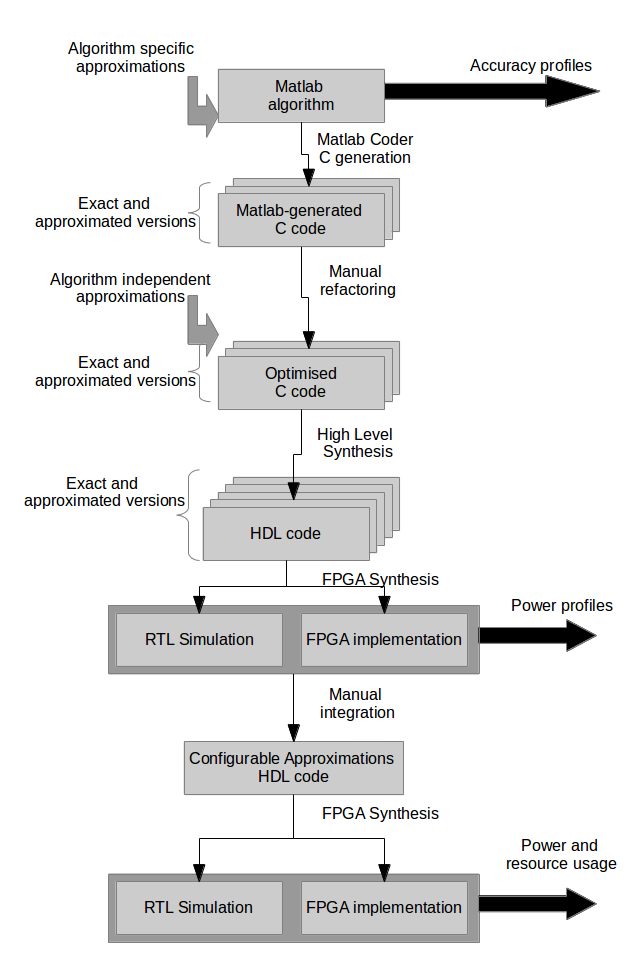
\includegraphics[width=0.9\columnwidth]{img/experimental_flow.png}
  \caption{Experimental design flow.}
  \label{fig:experimental_flow}
\end{figure}
